\documentclass[spec, och, otchet, hidelinks]{SCWorks}
% параметр - тип обучения - одно из значений:
%    spec     - специальность
%    bachelor - бакалавриат (по умолчанию)
%    master   - магистратура
% параметр - форма обучения - одно из значений:
%    och   - очное (по умолчанию)
%    zaoch - заочное
% параметр - тип работы - одно из значений:
%    otchet
%    referat    - реферат
%    coursework - курсовая работа (по умолчанию)
%    diploma    - дипломная работа
%    pract      - отчет по практике
%    pract      - отчет о научно-исследовательской работе
%    autoref    - автореферат выпускной работы
%    assignment - задание на выпускную квалификационную работу
%    review     - отзыв руководителя
%    critique   - рецензия на выпускную работу
% параметр - включение шрифта
%    times    - включение шрифта Times New Roman (если установлен)
%               по умолчанию выключен
\usepackage[T2A]{fontenc}
\usepackage[utf8]{inputenc}
\usepackage{graphicx}

\usepackage[sort,compress]{cite}
\usepackage{amsmath}
\usepackage{amssymb}
\usepackage{amsthm}
\usepackage{fancyvrb}
\usepackage{longtable}
\usepackage{array}
\usepackage[english,russian]{babel}
\usepackage{minted}
% Используется автором репозитория
%\usemintedstyle{xcode}
% Этот пакет включает в себя аналогичный Times New Roman шрифт.
% Необходим для успешной компиляции для UNIX-систем ввиду отсутствия TNR в нем.
% Можно использовать и для Windows.
\usepackage{tempora}


\usepackage[colorlinks=false]{hyperref}

\graphicspath{{figures/}}

\newcommand{\eqdef}{\stackrel {\rm def}{=}}

\usepackage{stackengine}
\newcommand\xrowht[2][0]{\addstackgap[.5\dimexpr#2\relax]{\vphantom{#1}}}

\newtheorem{lem}{Лемма}

% % При использовании biblatex вместо bibtex
%\usepackage[style=gost-numeric]{biblatex}
%\addbibresource{thesis.bib}

\begin{document}

% Кафедра (в родительном падеже)
\chair{математической кибернетики и компьютерных наук}

% Тема работы
\title{Преобразователи кодов}

% Курс
\course{3}

% Группа
\group{331}

% Факультет (в родительном падеже) (по умолчанию "факультета КНиИТ")
%\department{факультета КНиИТ}

% Специальность/направление код - наименование
%\napravlenie{02.03.02 "--- Фундаментальная информатика и информационные технологии}
%\napravlenie{02.03.01 "--- Математическое обеспечение и администрирование информационных систем}
%\napravlenie{09.03.01 "--- Информатика и вычислительная техника}
%\napravlenie{09.03.04 "--- Программная инженерия}
\napravlenie{10.05.01 "--- Компьютерная безопасность}

% Для студентки. Для работы студента следующая команда не нужна.
%\studenttitle{Студентки}

% Фамилия, имя, отчество в родительном падеже
\author{Бородина Артёма Горовича}

% Заведующий кафедрой
\chtitle{доцент, к.\,ф.-м.\,н.} % степень, звание
\chname{С.\,В.\,Миронов}

%Научный руководитель (для реферата преподаватель проверяющий работу)
\satitle{аспирант}%, к.\,ф.-м.\,н.} %должность, степень, звание
\saname{А.\,А.\,Мартышкин}

% Руководитель практики от организации (только для практики,
% для остальных типов работ не используется)
\patitle{к.\,ф.-м.\,н., доцент}
\paname{Д.\,Ю.\,Петров}

% Семестр (только для практики, для остальных
% типов работ не используется)
\term{2}

% Наименование практики (только для практики, для остальных
% типов работ не используется)
\practtype{учебная}

% Продолжительность практики (количество недель) (только для практики,
% для остальных типов работ не используется)
\duration{2}

% Даты начала и окончания практики (только для практики, для остальных
% типов работ не используется)
\practStart{01.07.2016}
\practFinish{14.07.2016}

% Год выполнения отчета
\date{2022}

\maketitle

% Включение нумерации рисунков, формул и таблиц по разделам
% (по умолчанию - нумерация сквозная)
% (допускается оба вида нумерации)
%\secNumbering


\tableofcontents

% Раздел "Обозначения и сокращения". Может отсутствовать в работе
% \abbreviations
% \begin{description}
%     \item ... "--- ...
%     \item ... "--- ...
% \end{description}

% Раздел "Определения". Может отсутствовать в работе
%\definitions

% Раздел "Определения, обозначения и сокращения". Может отсутствовать в работе.
% Если присутствует, то заменяет собой разделы "Обозначения и сокращения" и "Определения"
%\defabbr


% Раздел "Введение"

\intro

\par В ходе данной лабораторной работы мы ознакомимся с основными 
характеристиками интегральных преобразователей кодов (дешифратора, шифратора, 
демультиплексора и мультиплексора) и испытаем эти устройства.

\newpage

\section*{Задание 1.}
\addcontentsline{toc}{section}{Задание 1}

\par Запустить лабораторный комплекс Labworks и среду МS10. Открыть файл 
\textbf{30.6.ms10}, размещенный в папке \textbf{Circuit Design Suitе 10.0} 
среды МS10, или собрать на рабочем поле среды MS10 схему для испытания дешифратора 
\textbf{DC} и установить в диалоговых окнах компонентов их параметры или режимы 
работы. \textbf{Скопировать} схему на страницу отчета.

\begin{figure}[h]
	\center{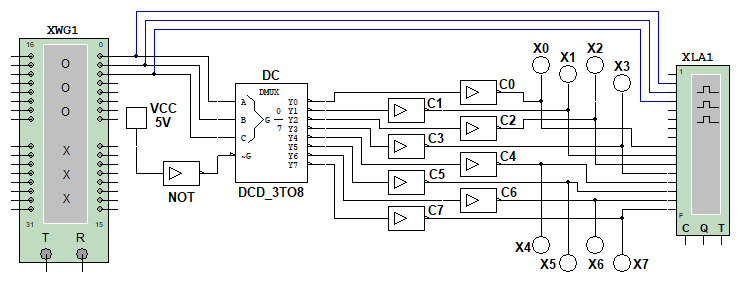
\includegraphics[scale=0.8]{dc.png}}
	\caption{Схема дешифратора.}
\end{figure}

\par \textbf{Запустить} программу моделирования дешифратора. Последовательно 
\textbf{подавать} на вход дешифратора логические слова. \textbf{Убедиться}, что при 
подаче на вход дешифратора каждой новой двоичной кодовой комбинации засвечивается 
только один пробник, который «распознает» свой входной код.

\newpage

\par Действительно, при подаче на вход дешифратора новой двоичной последовательности, 
засвечивается тот пробник, который распознаёт соответствующий код. Так, например для 
последовательности, состоящей из 32 нулей, загорится синий индикатор:

\begin{figure}[h]
	\center{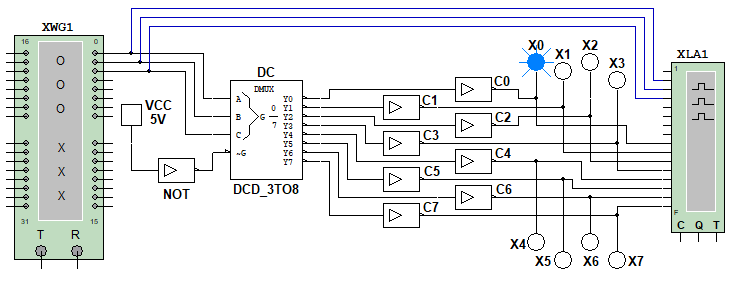
\includegraphics[scale=0.8]{blue_light.png}}
	\caption{Распознавание последовательности синим индикатором.}
\end{figure}

\par Для последовательности, состоящей из 31 нуля и 1 единицы, загорится зелёный индикатор:

\begin{figure}[h]
	\center{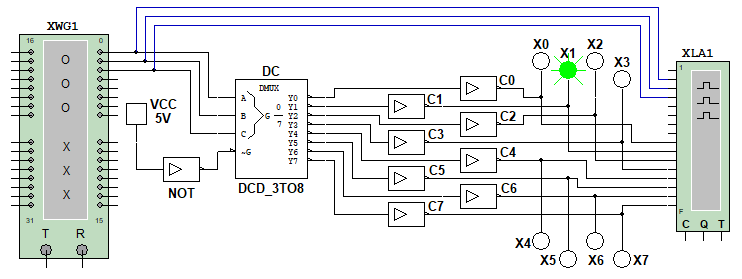
\includegraphics[scale=0.8]{green_light.png}}
	\caption{Распознавание последовательности зелёным индикатором.}
\end{figure}

\newpage

\par \textbf{Скопировать} временные диаграммы входных и выходных сигналов дешифратора
на страницу отчета. 

\begin{figure}[h]
	\center{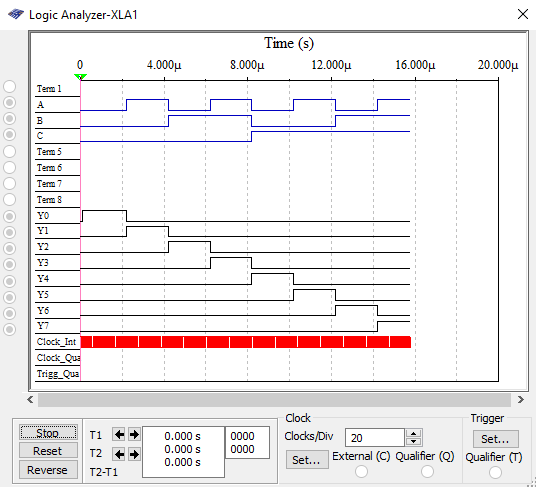
\includegraphics{diagrams.png}}
	\caption{Временные диаграммы входных и выходных сигналов дешифратора.}
\end{figure}

\par По результатам моделирования \textbf{составить} и \textbf{заполнить} таблицу переключений 
(функций $ Y_i = (A_iB_iC_i; \, G_i)) $ на выходах дешифратора \textbf{DC} 3х8.

\begin{table}[h!]
	\captionsetup{justification=centering}
	\begin{tabular}{|c|c|c|c|c|c|c|c|c|}
		\hline\xrowht[()]{10pt}
		$ A_i $ & $ \; 0 \; $ & $\; 1 \; $ & $ \; 0 \; $ & $ \; 1 \; $ & $ \; 0 \; $ & 
		$ \; 1 \; $ & $ \; 0 \; $ & $ \; 1 \; $ \\
		\hline\xrowht[()]{10pt}
		$ B_i \; $ & 0 & 0 & 1 & 1 & 0 & 0 & 1 & 1 \\
		\hline\xrowht[()]{10pt}
		$ C_i \; $ & 0 & 0 & 0 & 0 & 1 & 1 & 1 & 1 \\
		\hline\xrowht[()]{10pt}
		$ G_i $ & $ (0; 2) \mu $ & $ (2; 4) \mu $ & $ (4; 6) \mu $ & $ (6; 8) \mu $ & 
		$ (8; 10) \mu $ & $ (10; 12) \mu $ & $ (12; 14) \mu $ & $ (14; 16) \mu $ \\
		\hline		
	\end{tabular}
	\caption{Таблица переключений функций $ Y_i = (A_iB_iC_i; \, G_i)) $.} 
\end{table}

\newpage 

\section*{Задание 2.}
\addcontentsline{toc}{section}{Задание 2}

\par Открыть файл \textbf{30.8.ms10}, размещенный в папке 
\textbf{Circuit Design Suitе 10.0} среды МS10, или собрать на рабочем поле 
среды MS10 схему для испытания шифратора \textbf{СD} и установить в диалоговых окнах 
компонентов их параметры или режимы работы. \textbf{Скопировать} схему на страницу отчета.

\begin{figure}[h]
	\center{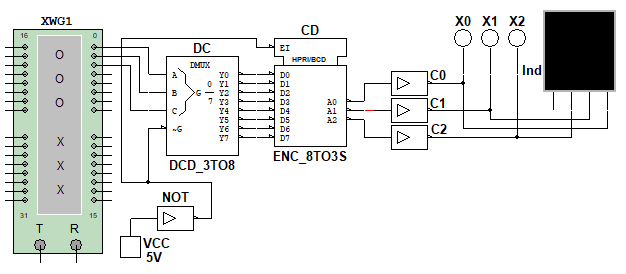
\includegraphics{cd.png}}
	\caption{Схема шифратора.}
\end{figure}

\newpage

\par \textbf{Запустить} программу моделирования шифратора. Последовательно 
\textbf{подавать} на вход дешифратора логические слова. \textbf{Убедиться}, что при 
подаче с выхода \textbf{DC} на вход шифратора \textbf{СD} 8-разрядной 
последовательности, в которой только одна позиция занята единицей, а остальные 
– нулями, на выходе шифратора формируются 3-разрядные двоичные коды 
\textbf{A0A1A2}, где \textbf{А0 = А}, \textbf{А1 = В} и \textbf{А2 = С}, 
соответствующие двоичным кодовым комбинациям на входе дешифратора \textbf{DC}.

\begin{figure}[h]
	\center{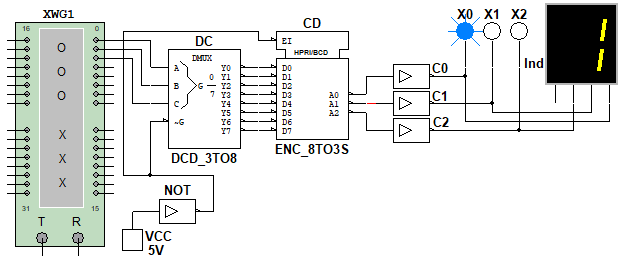
\includegraphics{one_is_given.png}}
	\caption{Подача на вход шифратора последовательности 00000001.}
\end{figure}

\begin{figure}[h]
	\center{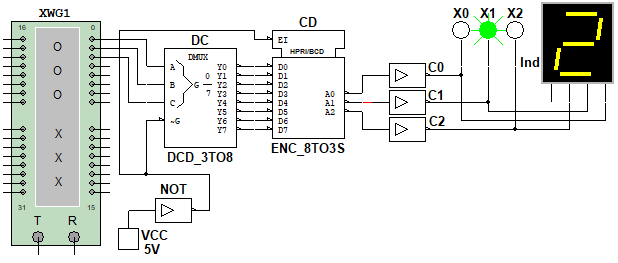
\includegraphics{two_is_given.png}}
	\caption{Подача на вход шифратора последовательности 00000010.}
\end{figure}

\newpage

\begin{figure}[h]
	\center{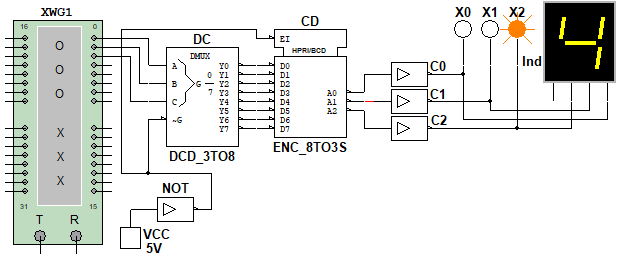
\includegraphics{four_is_given.png}}
	\caption{Подача на вход шифратора последовательности 00000100.}
\end{figure}

\par По результатам моделирования \textbf{составить} и \textbf{заполнить} таблицу
переключений на выходе шифратора \textbf{CD} 8х3.

\begin{table}[h!]
	\captionsetup{justification=centering}
	\centering
	\begin{tabular}{|c|c|c|c|c|c|c|c|c|}
		\hline\xrowht[()]{10pt}
		& $ \quad \emptyset \quad $ & $ \; X_0 \; $ & $ \; X_1 \; $ & $ \; X_0X_1 \; $ & $ \; X_2 \; $ &
		$ \; X_0X_2 \; $ & $ \; X_1X_2 \; $ & $ \; X_0X_1X_2 \; $ \\
		\hline\xrowht[()]{10pt}
		$ A_i \; $ & 0 & 0 & 0 & 0 & 1 & 1 & 1 & 1 \\
		\hline\xrowht[()]{10pt}
		$ B_i \; $ & 0 & 0 & 1 & 1 & 0 & 0 & 1 & 1 \\
		\hline\xrowht[()]{10pt}
		$ C_i \; $ & 0 & 1 & 0 & 1 & 0 & 1 & 0 & 1 \\
		\hline
	\end{tabular}
	\caption{Таблица переключений на выходе шифратора.} 
\end{table}

\newpage

\par \textbf{Преобразовать} схему дешифратора \textbf{DC} 3х8 и шифратора 
\textbf{CD} 8х3 в схему \textbf{DC} 2х4 и шифратора \textbf{CD} 4х2, отсоединив 
провод \textbf{С}, подходящий к дешифратору, и провод \textbf{A2} с выхода шифратора, 
и \textbf{составить} таблицы переключений дешифратора 2х4 и шифратора 4х2.

\begin{figure}[h]
	\center{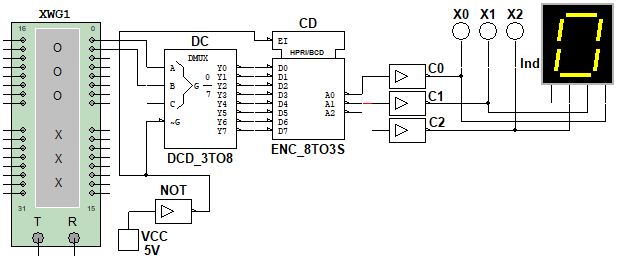
\includegraphics{dc_cd_transformation.png}}
	\caption{Преобразование декодера и кодера.}
\end{figure}

\begin{table}[h!]
	\captionsetup{justification=centering}
	\centering
	\begin{tabular}{|c|c|c|c|c|c|c|c|c|}
		\hline\xrowht[()]{10pt}
		& $ \quad \emptyset \quad $ & $ \; X_0 \; $ & $ \; X_1 \; $ & $ \; X_0X_1 \; $ & 
		$ \quad \emptyset \quad $ & $ \; X_0 \; $ & $ \; X_1 \; $ & $ \; X_0X_1 \; $ \\
		\hline\xrowht[()]{10pt}
		$ A_i \; $ & 0 & 0 & 0 & 0 & 1 & 1 & 1 & 1 \\
		\hline\xrowht[()]{10pt}
		$ B_i \; $ & 0 & 0 & 1 & 1 & 0 & 0 & 1 & 1 \\
		\hline\xrowht[()]{10pt}
		$ C_i \; $ & 0 & 1 & 0 & 1 & 0 & 1 & 0 & 1 \\
		\hline
	\end{tabular}
	\caption{Таблица переключений на выходе преобразованного шифратора.} 
\end{table}

\newpage

\section*{Задание 3.}
\addcontentsline{toc}{section}{Задание 3}

\par Открыть файл \textbf{30.9.ms10}, размещенный в папке 
\textbf{Circuit Design Suitе 10.0} среды МS10, или собрать на рабочем поле среды MS10 
схему для испытания \textit{демультиплексора} \textbf{DMS} и установить в диалоговых 
окнах компонентов их параметры или режимы работы.

\par Для обеспечения медленного перемещения лучей на экране анализатора
\textbf{XLA1 установить} частоту его таймера $ f_a $ = 500 Гц и число импульсов, 
приходящихся на одно деление, \textbf{Clocs/div} = 80.

\begin{figure}[h]
	\center{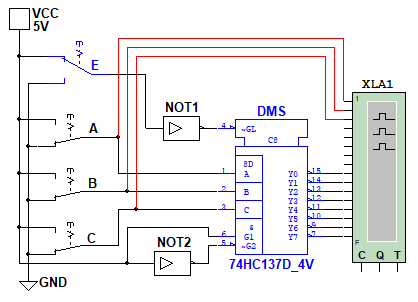
\includegraphics{dms.png}}
	\caption{Схема демультиплексора.}
\end{figure}

\par \textbf{Задать} код ключей 111 и \textbf{щелкнуть} мышью на кнопке \textbf{Run/Stop}. Кривые адресных
и выходных логических сигналов медленно разворачиваются во времени на экране анализатора.

\textbf{Остановить} процесс моделирования при приближении лучей анализатора к линии разметки экрана.

\par Повторять перечисленные выше операции для спадающих счетных комбинаций адресных сигналов (с 110 до 000) 
до тех пор, пока не будет записан процесс моделирования при адресном слове 000.

\newpage

\textbf{Скопировать} схему и временные диаграммы входных и выходных сиг-
налов на страницу отчета.

\begin{figure}[h]
	\center{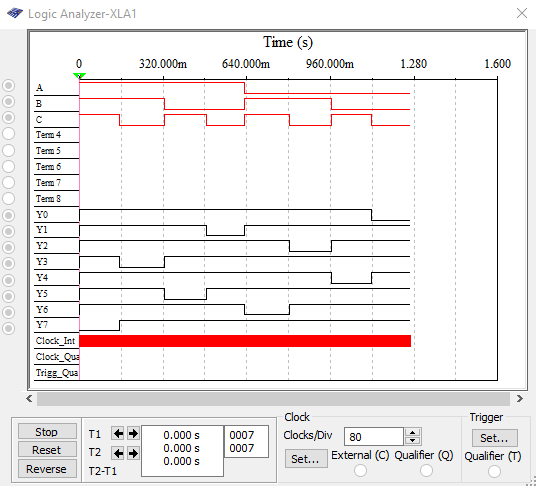
\includegraphics{dms_diagrams.png}}
	\caption{Временные диаграммы входных и выходных сигналов.}
\end{figure}

\newpage

\section*{Задание 4.}
\addcontentsline{toc}{section}{Задание 4}

\par Открыть файл \textbf{30.10.ms10}, размещенный в папке \textbf{Circuit Design Suitе 10.0} 
среды МS10, или собрать на рабочем поле среды MS10 схему для испытания \textit{демультиплексора} 
\textbf{DMS} 1х16 и установить в диалоговых окнах компонентов их параметры или режимы работы.
\textbf{Скопировать} схему в отчет.

\begin{figure}[h]
	\center{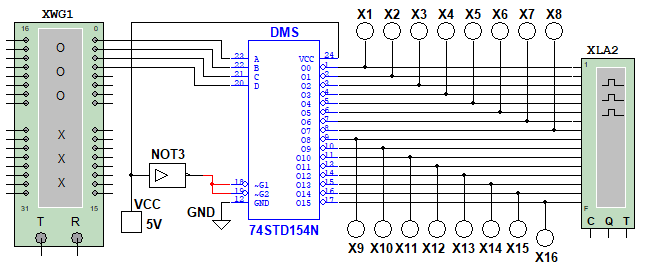
\includegraphics{dms_task_four.png}}
	\caption{Временные диаграммы входных и выходных сигналов.}
\end{figure}

\par \textbf{Запустить} программу моделирования демультиплексора \textbf{DMS} 1x16. Последовательно 
подавать на вход демультиплексора логические слова, начиная с комбинации 0000 адресного сигнала и 
заканчивая комбинацией 1111, и \textbf{наблюдать} за изменениями выходных сигналов по показаниям 
индикаторов и в окне анализатора \textbf{XLA2}.

\newpage

\par \textbf{Скопировать} на страницу отчета временные диаграммы выходных сигналов де-
мультиплексора \textbf{DMS} 1х16.

\begin{figure}[h]
	\center{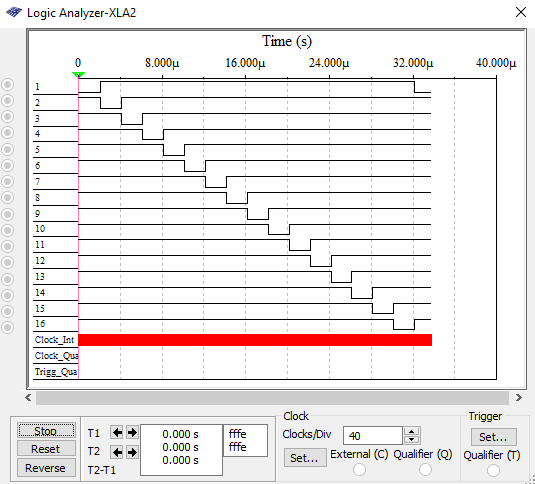
\includegraphics{dms_task_four_diagrams.png}}
	\caption{Временные диаграммы выходных сигналов демультиплексора.}
\end{figure}

\newpage

\section*{Задание 5.}
\addcontentsline{toc}{section}{Задание 5}

\par Открыть файл \textbf{30.12.ms10}, размещенный в папке \textbf{Circuit Design Suitе 10.0} среды МS10, 
или собрать на рабочем поле среды MS10 схему для испытания \textit{мультиплексора} \textbf{MS} 8х1 и 
установить в диалоговых окнах компонентов их параметры или режимы работы. \textbf{Скопировать} 
схему в отчет.

\begin{figure}[h]
	\center{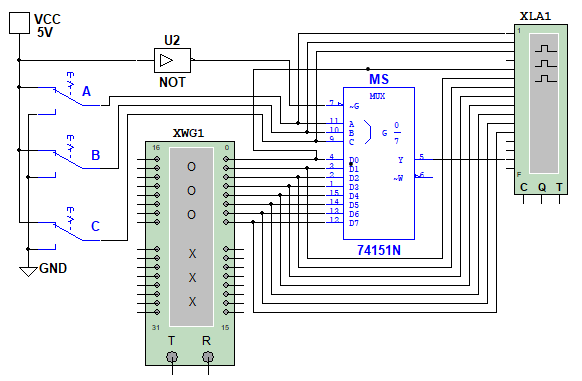
\includegraphics{ms.png}}
	\caption{Схема мультиплексора.}
\end{figure}

\newpage

\par \textbf{Записать} в первые восемь ячеек памяти генератора XWG1 произвольные 8-разрядные кодовые 
слова, задать частоту $ f_{\Gamma} $ = 500 кГц и режим \textbf{Step} его работы.

\begin{figure}[h]
	\center{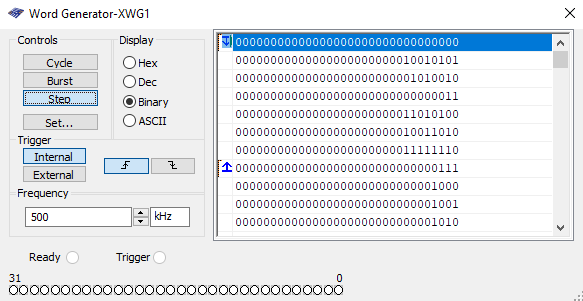
\includegraphics{generator_params.png}}
	\caption{Установка параметров работы генератора.}
\end{figure}

\par \textbf{Задать} частоту $ f_a $ = 20 МГц таймера логического анализатора \textbf{XLA1} и количество 
импульсов таймера \textbf{Clock/div} = 20, приходящихся на одно деление.

\begin{figure}[h]
	\center{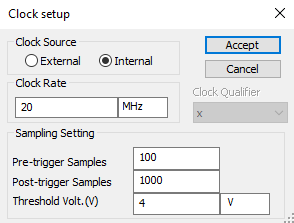
\includegraphics{clock_setup.png}}
	\caption{Установка параметров работы таймера логического анализатора.}
\end{figure}

\newpage

\textbf{Установить} с помощью ключей \textbf{А, В} и \textbf{С} адресный код (был установлен 
адресный код $ 110_2 $), и \textbf{запустить} программу моделирования мультиплексора. 
\textbf{Получить} и \textbf{скопировать} временные диаграммы входных сигналов 
\textbf{D0, D1, $ \dots $, D7} и выходного сигнала \textbf{Y} мультиплексора на страницу отчета.

\begin{figure}[h]
	\center{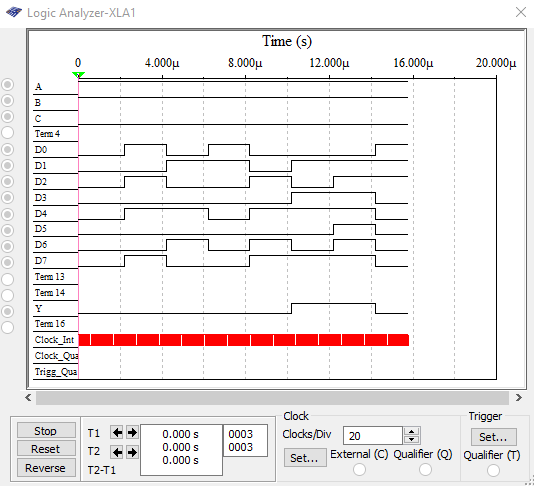
\includegraphics{diagrams_task_five.png}}
	\caption{Временные диаграммы входных сигналов \textbf{D0, D1, $ \dots $, D7} и выходного сигнала 
		\textbf{Y}.}
\end{figure}

\newpage

\section*{Тестовые задания.}
\addcontentsline{toc}{section}{Тестовые задания}

\par \textbf{1}. Укажите \textbf{задачи}:
\par а) для демультиплексирования данных и адресной логики в запоминающих устройствах, а также для 
преобразования двоично-десятичного кода в десятичный с целью управления индикаторными и печатающими 
устройствами;

\par б) для преобразования десятичных чисел в двоичные или в двоично-десятичный код, например, в 
микрокалькуляторах, в которых нажатие десятичных клавишей соответствует генерации соответствующего 
двоичного кода;

\par в) для хранения и преобразования многоразрядных двоичных чисел;

\par г) для коммутации в заданном порядке сигналов, поступающих с нескольких входных шин на одну выходную;

\par д) для распределения в требуемой последовательности по нескольким выходам сигналов с одного 
информационного входа, в частности для передачи информации по одной линии от нескольких установленных 
на ней датчиков, \\
при решении которых используется: \\
шифратор: \textbf{б}; \\
дешифратор: \textbf{а}; \\
мультиплексор: \textbf{г}; \\
демультиплексор: \textbf{д}. \\

\par \textbf{2}. Укажите, \textbf{с какого разряда} бинарного слова генератора XWG будет передаваться 
информация на выход мультиплексора 8х3 при адресном коде 100 на его входе: \textbf{7}. \\

\par \textbf{3}. Укажите число \textbf{выходов} дешифратора при трех информационных входах: \textbf{8}. \\

\newpage

\par \textbf{4}. Укажите назначение \textbf{стробирующих} входов в преобразователях кодов:
\par $ \square \; $ для увеличения числа коммутируемых информационных входов, а также для блокирования 
работы преобразователей; \\

\par \textbf{5}. Укажите, в каком \textbf{преобразователе} выбор входа по его номеру (адресу) 
осуществляется с помощью двоичного кода: \textbf{мультиплексор}. \\

\par \textbf{6} Укажите \textbf{число выводов} у шифратора при четырех информационных входах: 
\textbf{2}. \\

\par \textbf{7} Укажите, какой из приведенных преобразователей кодов выпускается промышленностью только 
в \textbf{составе других устройств}: \textbf{демультиплексоры} как таковые промышленностью не 
выпускаются, поскольку режим мультиплексирования может быть реализован как частный случай в других 
устройствах - в дешифраторах.

\newpage

\conclusion

\par В ходе данной лабораторной работы мы ознакомились с основными характеристиками интегральных 
преобразователей кодов (дешифратора, шифратора, демультиплексора и мультиплексора) 
и испытали эти устройства путём составления диаграмм их входных и выходных сигналов.

\end{document}